\chapter{Auswertung}
\section{Statistiken und Vergleiche der Pathfinding-Algorithmen}
\begin{center}
  \boxed{
    \textit{Alle notierten Messresultate pro Vergleich befinden sich im Anhang dieser Arbeit.}
  }
\end{center}

Das Autorenteam hat sich auf eine Rastergrösse von $50\times 50$ Felder
entschieden und durchlief die Vergleiche $125$-mal. Die Rechenzeiten wurden
auf $0.1$ ms gerundet. Die Diagonalen wurden mitbeachtet, da dies zu
optimierten Strecken führen kann.

Die $125$ Versuche wurden zuerst in folgende Kategorien in den Resultate
unterteilt: Weg des kürzesten Pathfinders von 0-10 Felder, 11-20 Felder,
21-30 Felder, 31-40 Felder und 41-50 Felder. Jede dieser Unterteilung hat
25 Vergleichsergebnisse. Diese Unterteilung hat den Grund, dass auf
längeren Wege die Unterschiede nach der Erfahrung dieser Arbeit durch
das Autorenteam deutlicher zu sehen sind.

\begin{longtable}[]{@{}l@{}}
\toprule
\endhead
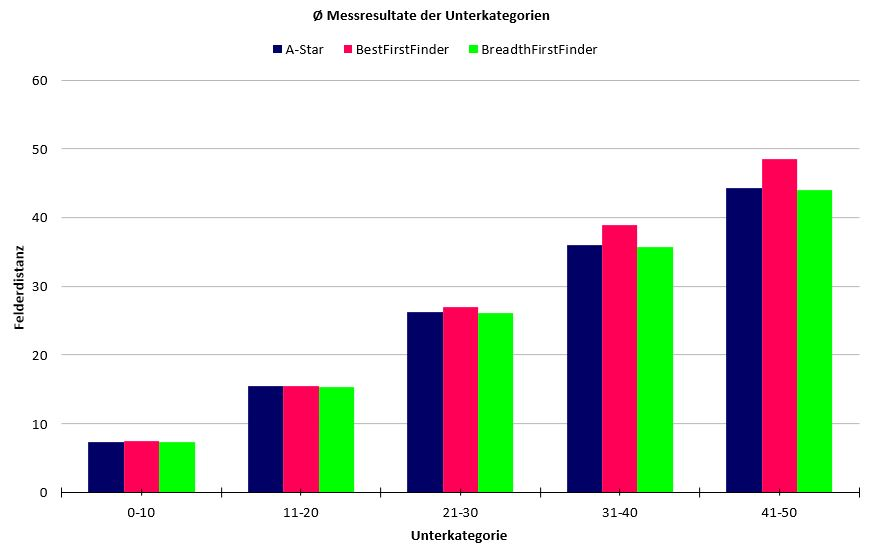
\includegraphics[width=6.26111in,height=4.02639in]{statistik_1.JPG}\tabularnewline
\bottomrule
\end{longtable}

Man erkennt gut, dass der A-Star und BreadthFirstFinder circa die gleiche
Felderdistanz finden. Je grösser der Abstand von Start und Ziel, desto grösser ist der Unterschied zwischen dem BestFirtFinder und den anderen zwei.

\begin{longtable}[]{@{}l@{}}
\toprule
\endhead
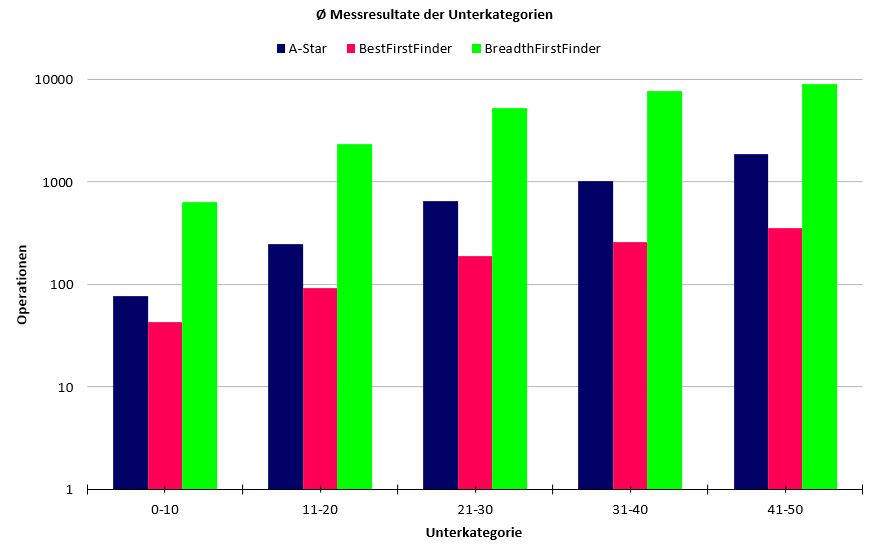
\includegraphics[width=6.26111in,height=3.95625in]{statistik_2.JPG}\tabularnewline
\bottomrule
\end{longtable}

Hierbei muss beachtet werden, dass die Diagrammdarstellung logarithmisch ist. Im Aufwand der
ausgeführten Operationen steigt der BreadthFirstFinder viel extremer als
die anderen. Der A-Star muss im Verhältnis zum BestFirstFinder immer
mehr Operationen ausführen. Die Steigung des BreadthFirstFinder senkt
sich im Laufe der Felderdistanz. Dies kommt daher, dass er am Rand des
Rasters ist und diese Seite nicht mehr weiter erkunden muss. Die
Vorteile einer Heuristik wird hier klar verdeutlicht. Der A-Star und
BestFirstFinder müssen durch die Wahrscheinlichkeitsberechnung weniger
Operationen durchführen.

\begin{longtable}[]{@{}l@{}}
\toprule
\endhead
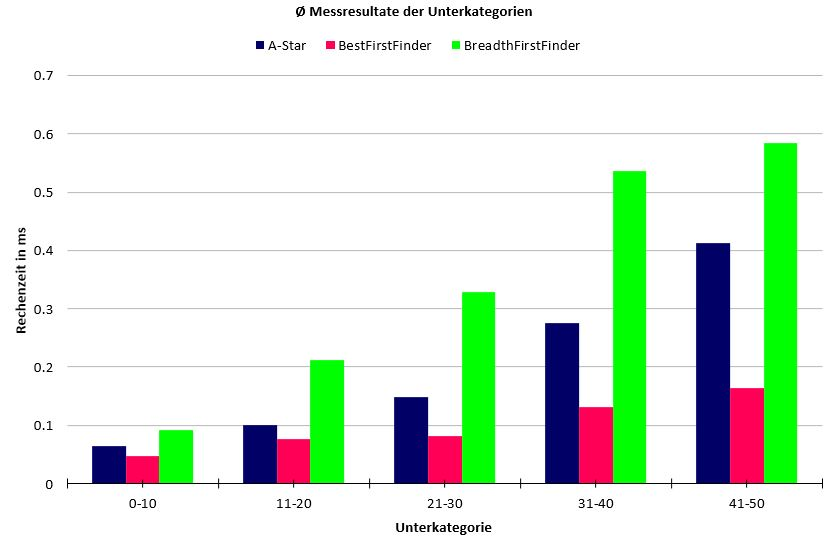
\includegraphics[width=6.26944in,height=4.15625in]{statistik_3.JPG}\tabularnewline
\bottomrule
\end{longtable}

Da der BestFirstFinder den erstbesten Weg tiefer durchsucht, ist seine
Rechenzeit um einiges kürzer als die anderen. Da der
BreadthFirstFinder am meisten Operationen hat, folgt, dass
seine Rechenzeit höher als die vom A-Star oder BestFirstFinder ist.

\section{Interpretation Resultate}

Aus den Statistiken kann man folgendes herauslesen:

\begin{itemize}
\item
  Der A-Star und BreadthFirstFinder finden ungefähr den gleich optimalen Weg,
  wobei der BreadthFirstFinder viel mehr an Operationen aufwenden muss,
  da er über keine Heuristik verfügt.
\item
  Hat man begrenzte Zeit, so ist der BestFirstFinder gut geeignet, er
  findet nicht den optimalsten Weg, spart dafür in Zeit und Operationen.
\item
  Je grösser das Raster, desto weniger ist der BreadthFirstFinder
  geeignet, da er zu viele Operationen benötigt und im Vergleich zum A-Star langsam wird.
\item
  Die Rechenzeit vom BestFirstFinder steigt linear und die vom
  A-Star und BreadthFirstFinder exponential, solange der
  BreadthFirstFinder keine Rasterseite erreicht hat.
\end{itemize}


\section{Zusammenfassung}
Es wurde beschrieben und erklärt, was ein Algorithmus und Pathfinding-Algorithmus ist. Es ist geklärt, wozu man Graphen braucht und wie diese in Pathfinding-Algorithmen einfliessen. Durch ein technisches Produkt werden die Unterschiede des A-Star, BestFirstFinde und BreadthFirstFidner in Vergleichen verdeutlicht. Die Realisierung der Webapplikation ist klar beschrieben und dessen Messresultate in statistischen Diagrammen verglichen und erläutert. Durch die Bearbeitung der Fachliteratur kam heraus, dass die benutzten Pathfinding-Algorithmen nicht aus einem Uralgorithmus stammen. Jeder der Algorithmen basiert auf einer Idee, wie das Vorgehen zum Lösen der Aufgabe bearbeitet werden soll. Der BreadthFirstFidner sucht ausschliesslich in der Breite der Graphen, das heisst er schaut sich alle ihm am nächstliegenden Graphen zuerst an. Der BestFirstFindes sucht in der Tiefe nach der Lösung und vernachlässigt potentiell bessere Lösungen, die am Anfang nicht besser aussehen. Der A-Star geht mit intelligenten Listen vor, mit denen er jeden Zyklus dem wahrscheinlich besten Graph als nächstes untersucht. Durch das erweiterte Produkt mit Vergleichsmöglichkeiten des selben Rasters konnten diese Schlüsse durch die Statistiken belegt werden. Interpretiert man die Resultate mit dem vorgegebenen Oberthema, erkennt man die daraus folgenden Erkenntnisse, wie die einzelnen Pathfinding-Algorithmen in ihren Merkmalen funktionieren und wie sie am besten anzuwenden sind. Ein Problem ist, dass diese Algorithmen in einem zweidimensionalen Raum funktionieren, unsere Welt jedoch dreidimensional ist. Hätte man komplexere dreidimensionale Pathfinding-Algorithmen untersucht, wäre der Aufwand zur Erkenntnis bestimmt höher und hätte mehr Einflüsse im Raum. Die Ortsbestimmung über ein GPS ist schwieriger als das berechnen einer Schachfigur auf einem Spielfeld durch Pathfinding-Algorithmen. Mit der Erkenntnis dieser Arbeit kann beispielsweise ein Spieleentwickler besser bestimmen, welchen Pathfinding-Algorithmus er für sein zweidimensionales Spiel wählen soll und warum.
